% Journal Quantum Science and Technology
% Special issue: Focus on Perspectives on the Future of Variational Quantum Computing
% https://iopscience.iop.org/collections/qst-241120-732


\documentclass[12pt]{iopart}

\newcommand{\gguide}{{\it Preparing graphics for IOP Publishing journals}}
%Uncomment next line if AMS fonts required
%\usepackage{iopams}  

\usepackage[hidelinks]{hyperref}
\usepackage{url}
\usepackage{comment}
\usepackage{graphicx}
\usepackage{float}
\usepackage{subfigure}
\usepackage{tabularx}
\usepackage{orcidlink}
\usepackage{cite}
\bibliographystyle{iopart-num}
\usepackage{amsmath}
\usepackage{appendix}



\begin{document}

%\title[Quantum Computing Plasma Dispersion Relations]{Quantum Computing Plasma Dispersion Relations}

\title[Plasma Dispersion Relations on Quantum Computers]{Plasma Dispersion Relations on Quantum Computers}


\author{
    Óscar Amaro \orcidlink{0000-0003-0615-0686} $^1$,
    Lucas Gamiz \orcidlink{0000-0002-7393-0896} $^1$, %Lucas Ivan Inigo Gamiz <lucas.inigo.gamiz@tecnico.ulisboa.pt>,
    Efstratios Koukoutsis \orcidlink{0000-0002-9143-2743} $^2$,
    Marija Vranic \orcidlink{0000-0003-3764-0645} $^1$ %marija.vranic@tecnico.ulisboa.pt
  }

\address{$^1$ GoLP/Instituto de Plasma e Fus\~ao Nuclear, Instituto Superior T\'ecnico, Universidade de Lisboa, Lisbon, Portugal\\
$^2$ School of Electrical and Computer Engineering,
National Technical University of Athens, Zographou 15780, Greece\\
}

%\address{
%GoLP/Instituto de Plasmas e Fus\~{a}o Nuclear, Instituto Superior T\'{e}cnico, Universidade de Lisboa, 1049-001 Lisbon, Portugal
%}
\ead{\footnotesize
\href{mailto:oscar.amaro@tecnico.ulisboa.pt}{oscar.amaro@tecnico.ulisboa.pt}, \href{mailto:marija.vranic@tecnico.ulisboa.pt}{marija.vranic@tecnico.ulisboa.pt}
}\normalsize

\vspace{10pt}

\begin{abstract}

Collecting raw results before going to the main

\end{abstract}


\section{Introduction}

Outline
\begin{itemize}
    \item Rodeo Alg and QPE for the cold plasma Hermitian setup 2qubits (+anc) on QPU
    \item Weibel Instability, SzNagy Dilation and Xie Variational ( (H-eps)dagger (H-eps) ) for non-Hermitian 2qubits (+anc) on QPU
    \item Krylov for larger Hermitian matrices (kinetic plasma) via the Hermite ladder
    \item appendix with toy-models for each method (possibly analytical results)
\end{itemize}

Literature review



\section{Cold Plasma: Rodeo, QPE}



\begin{figure}[!h]
    \centering
    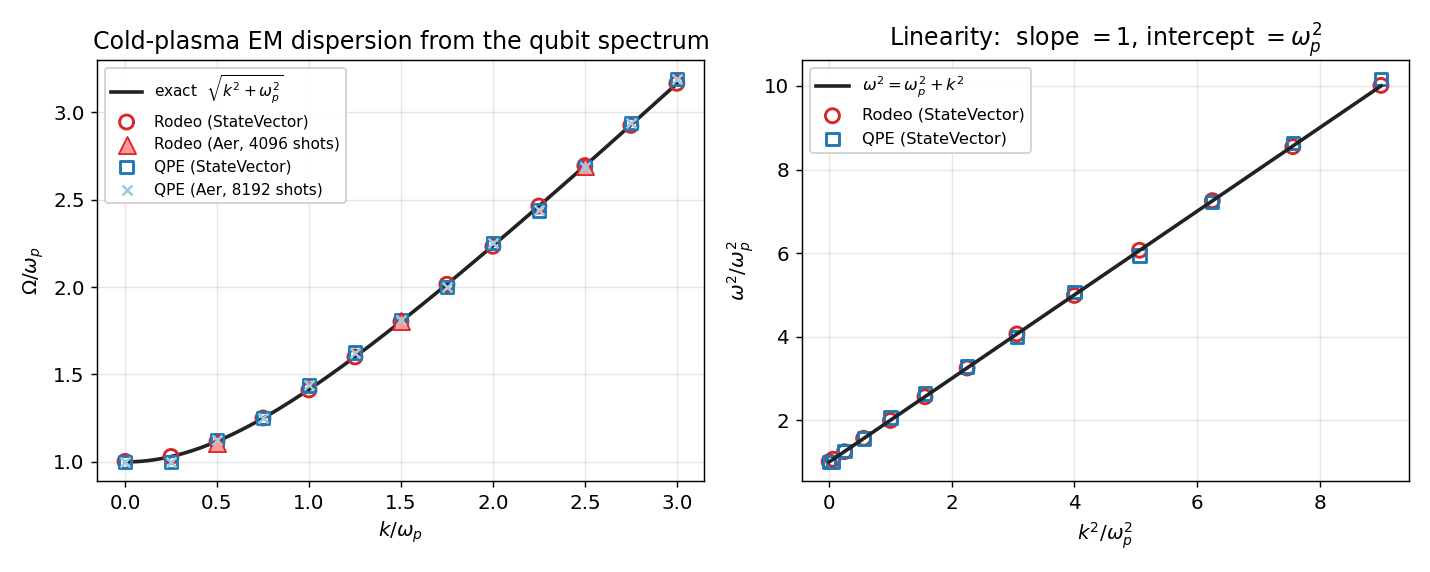
\includegraphics[width=0.8\linewidth]{figures_collect/1_cold_plasma/fig1_dispersion.png}
    \caption{1}
    \label{fig:ptsym_complex_plane}
\end{figure}


\begin{figure}[!h]
    \centering
    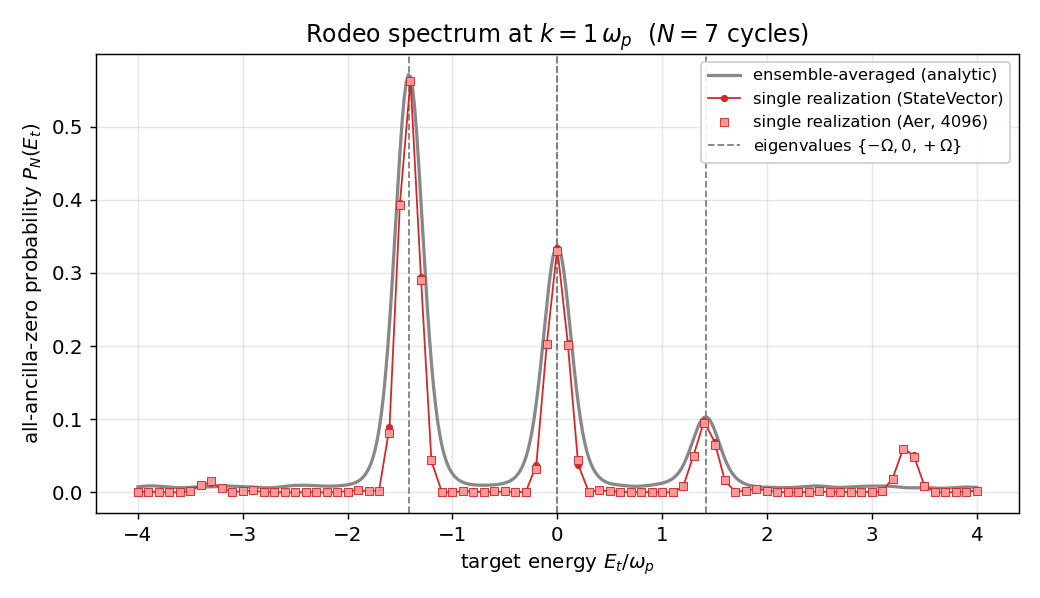
\includegraphics[width=0.65\linewidth]{figures_collect/1_cold_plasma/fig2_rodeo_scan.png}
    \caption{2}
    \label{fig:ptsym_complex_plane}
\end{figure}


\begin{figure}[!h]
    \centering
    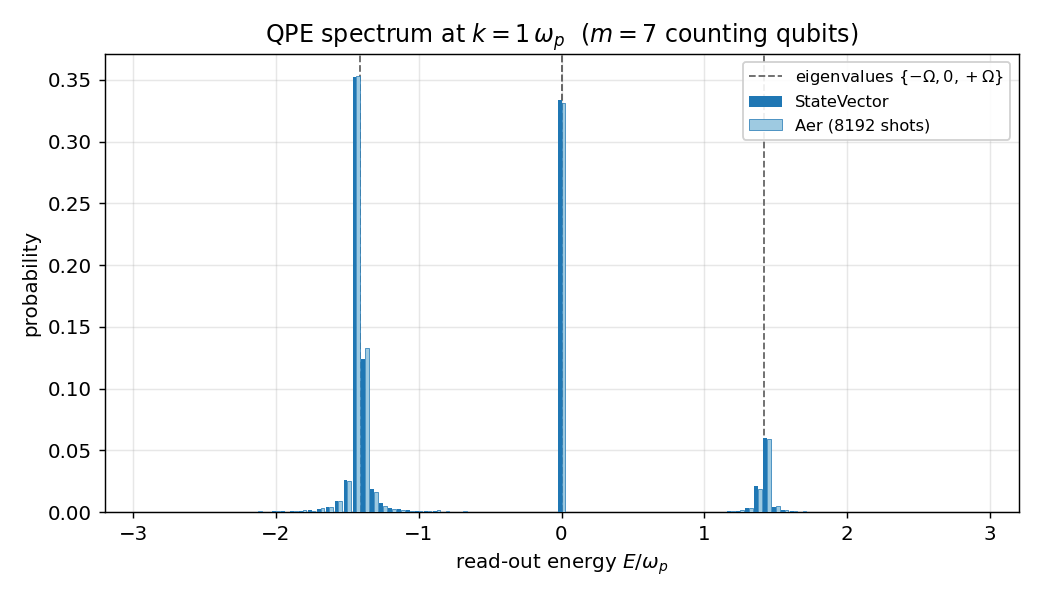
\includegraphics[width=0.65\linewidth]{figures_collect/1_cold_plasma/fig3_qpe_hist.png}
    \caption{3}
    \label{fig:ptsym_complex_plane}
\end{figure}


\begin{figure}[!h]
    \centering
    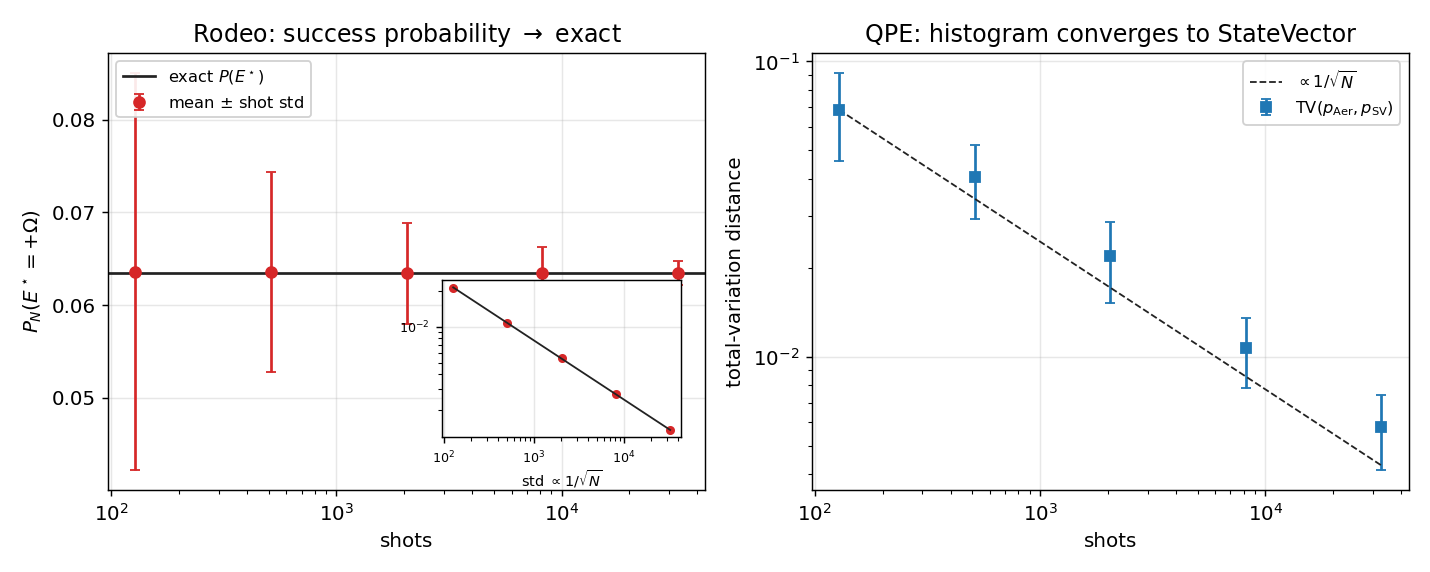
\includegraphics[width=0.8\linewidth]{figures_collect/1_cold_plasma/fig4_shot_convergence.png}
    \caption{4}
    \label{fig:ptsym_complex_plane}
\end{figure}


\begin{figure}[!h]
    \centering
    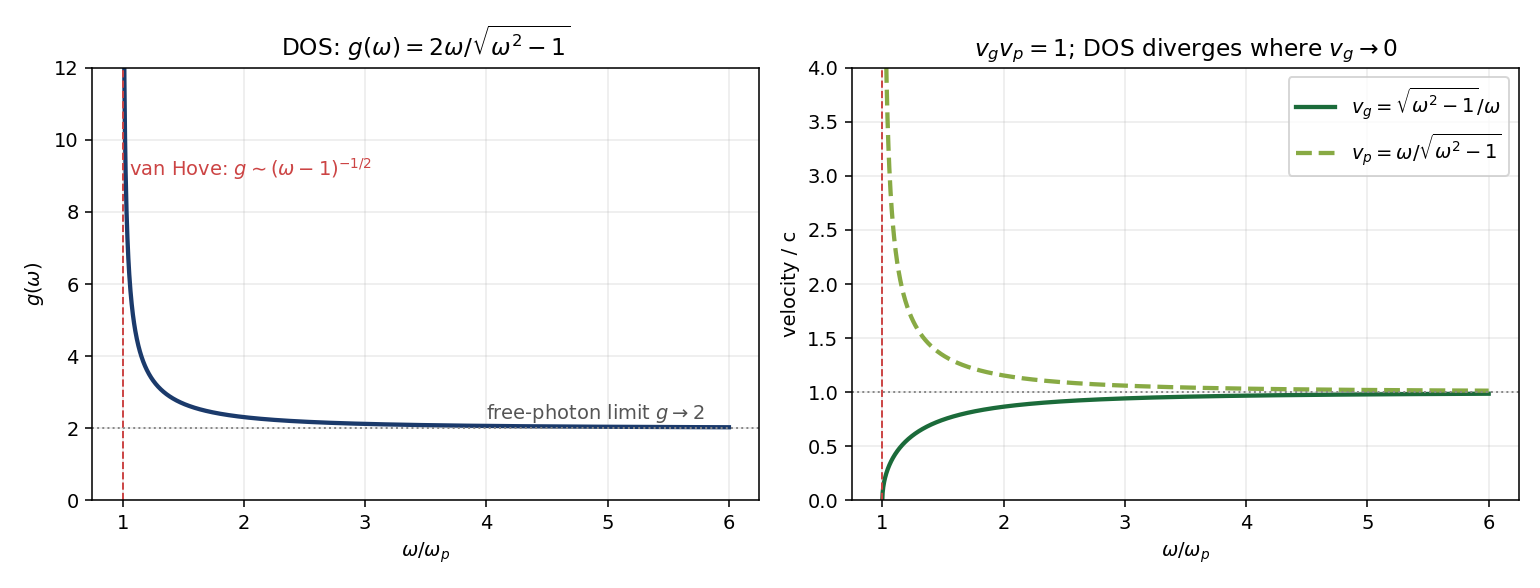
\includegraphics[width=0.65\linewidth]{figures_collect/1_cold_plasma/cold_plasma_dos.png}
    \caption{Density of states DOS}
    \label{fig:ptsym_complex_plane}
\end{figure}



\section{Weibel: SzNagy Dilation and Krylov }


\begin{figure}[!h]
    \centering
    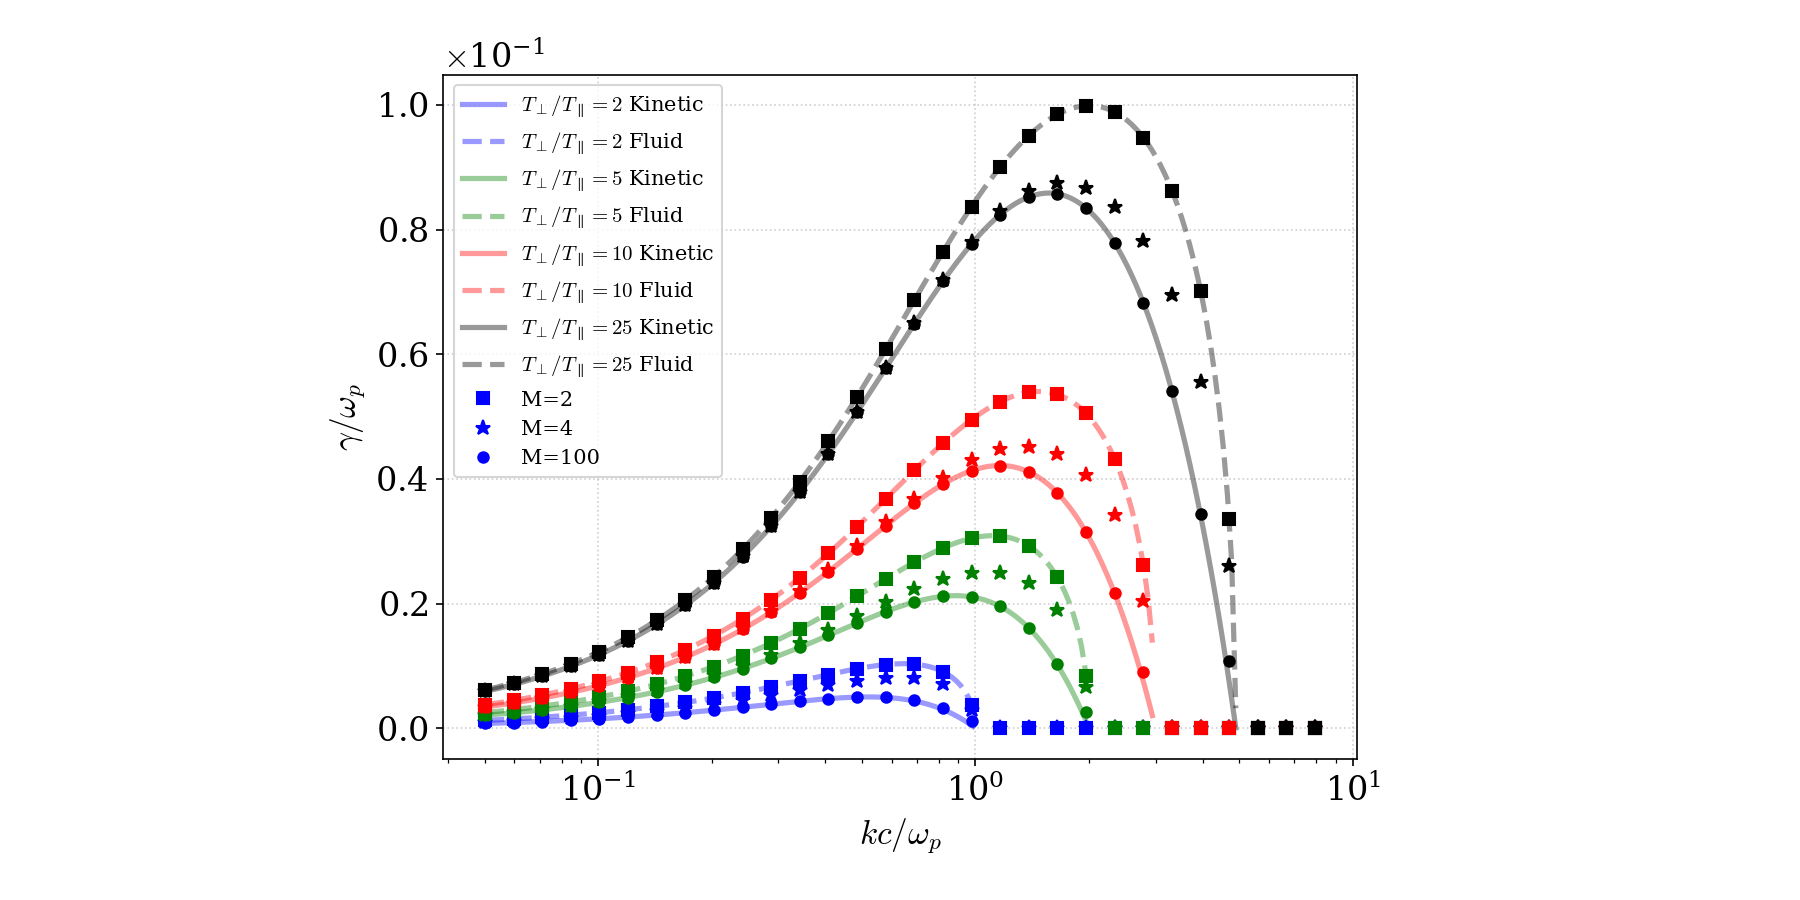
\includegraphics[width=0.8\linewidth]{figures_collect/2_weibel/weibel_hermite_dispersion.png}
    \caption{4}
    \label{fig:ptsym_complex_plane}
\end{figure}

\begin{figure}[!h]
    \centering
    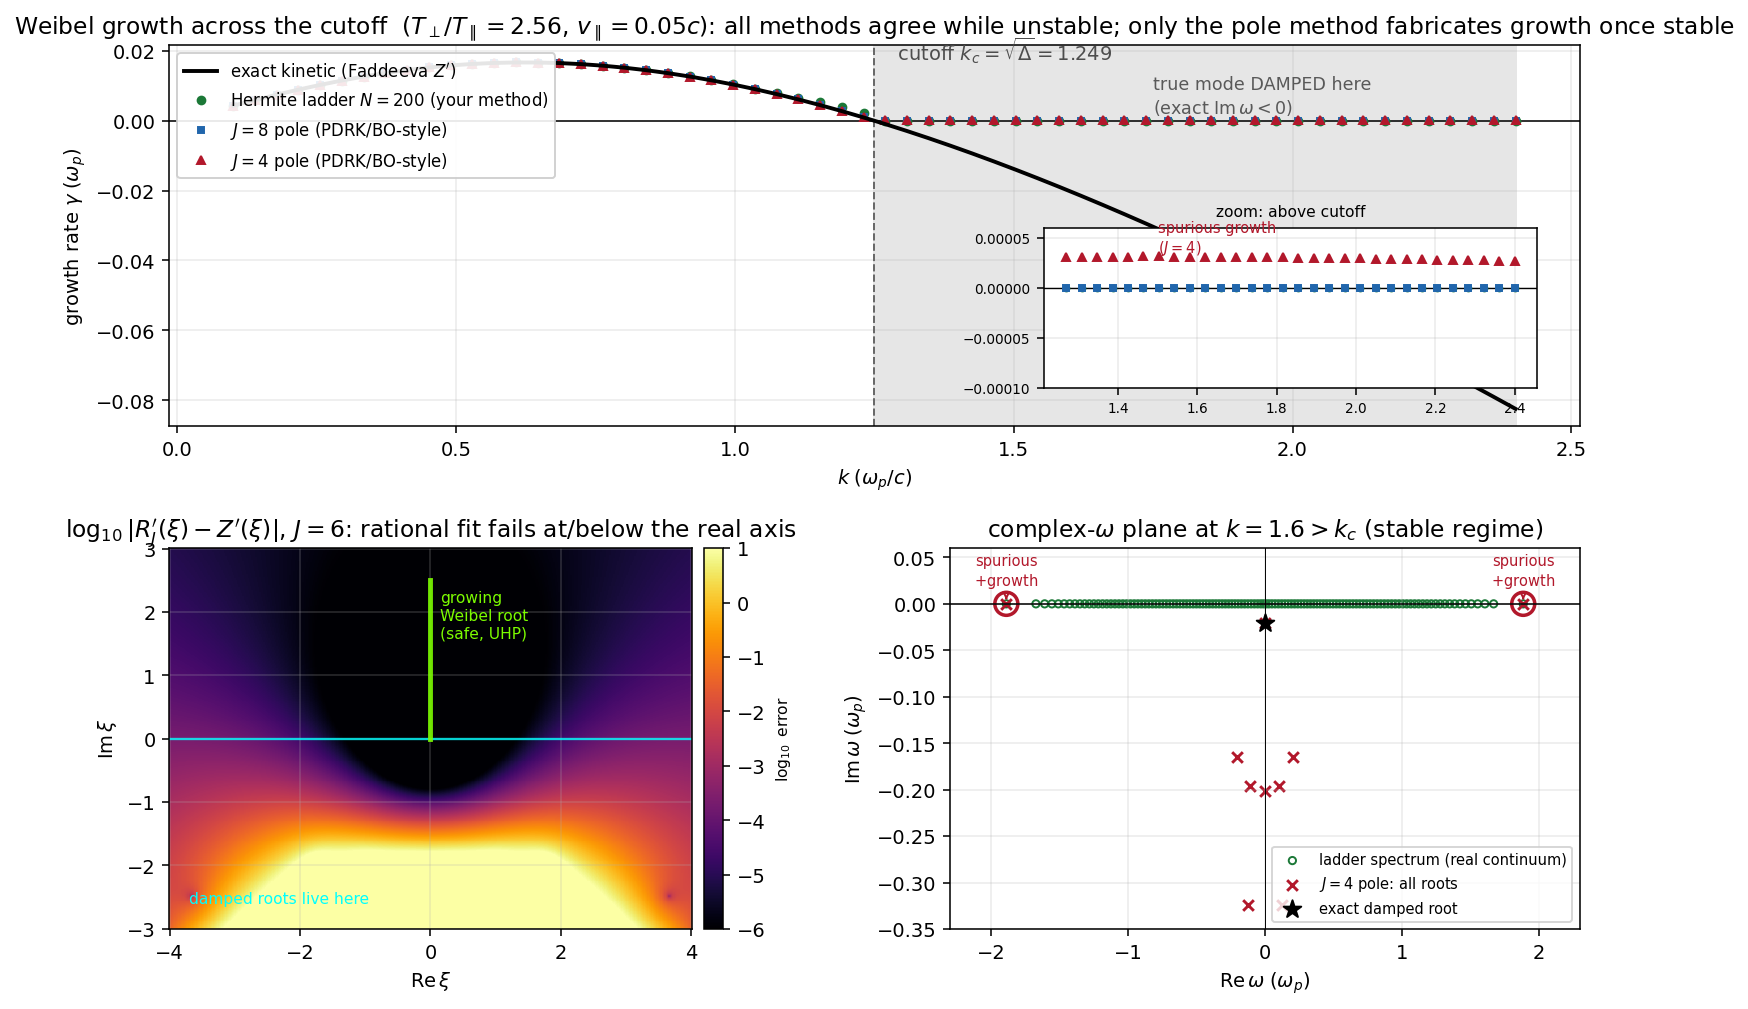
\includegraphics[width=0.8\linewidth]{figures_collect/2_weibel/weibel_benchmark.png}
    \caption{4}
    \label{fig:ptsym_complex_plane}
\end{figure}




\section{Hermite ladder, Krylov}




\end{document}